\documentclass[12pt,a4paper]{scrartcl}

\usepackage[a4paper, left=2cm, right=2cm, bottom=1cm, top=1cm, includeheadfoot]{geometry}
\usepackage[ngerman]{babel}
\usepackage[utf8]{inputenc} % comment this if you uncomment utf8x
%\usepackage[utf8x]{inputenc} % uncomment this if there are problems with 'ä', 'ü', 'ö'
\usepackage{ucs}
\usepackage[usenames,dvipsnames]{xcolor}
\usepackage[fleqn]{amsmath}
\usepackage{amsfonts}
\usepackage{amssymb}
\usepackage{color}
\usepackage{listings}
\usepackage{hyperref}
\usepackage{amsfonts}
\usepackage{listings}
\usepackage{scrpage2}
\usepackage{graphicx}
\usepackage{pdfpages}
\usepackage{mathtools}
\usepackage{multirow}
\usepackage{float}
\usepackage{matlab-prettifier}


\definecolor{mygray}{rgb}{0.9,0.9,0.9}
\lstset{language=[Visual]Basic, morekeywords={param, local}}


\lstset{
   literate={ö}{{\"o}}1
           {ä}{{\"a}}1
           {ü}{{\"u}}1
           {ß}{{\ss}}1
           {é}{{\'e}}1,
   inputencoding=ansinew,
   extendedchars=true,
   basicstyle=\scriptsize\ttfamily,
   numberstyle=\scriptsize,
   breaklines=true,
   tabsize=4,
   numbersep=5pt
}
\lstdefinestyle{customcpp}{
   language=C++,
   backgroundcolor=\color{mygray},
   numbers=left,
   keywordstyle=\color{blue}\bfseries,
   stringstyle=\color{BrickRed}\ttfamily,
   commentstyle=\color{OliveGreen}\ttfamily,
   showspaces=false,
   showstringspaces=false,
   showtabs=false
}
\lstdefinestyle{customoutput}{
   backgroundcolor=\color{mygray},
   numbers=none,
   showspaces=false,
   showtabs=false
}

\newcommand{\sourceCode}[1]{\lstinputlisting[style=customcpp]{#1}}
\begin{document}

\title{SCD5 - Matlab - Übung 3}
\date{09. November 2017}
\author{Daniel Klepatsch \and Thomas Reisinger}
        
\maketitle

\newpage

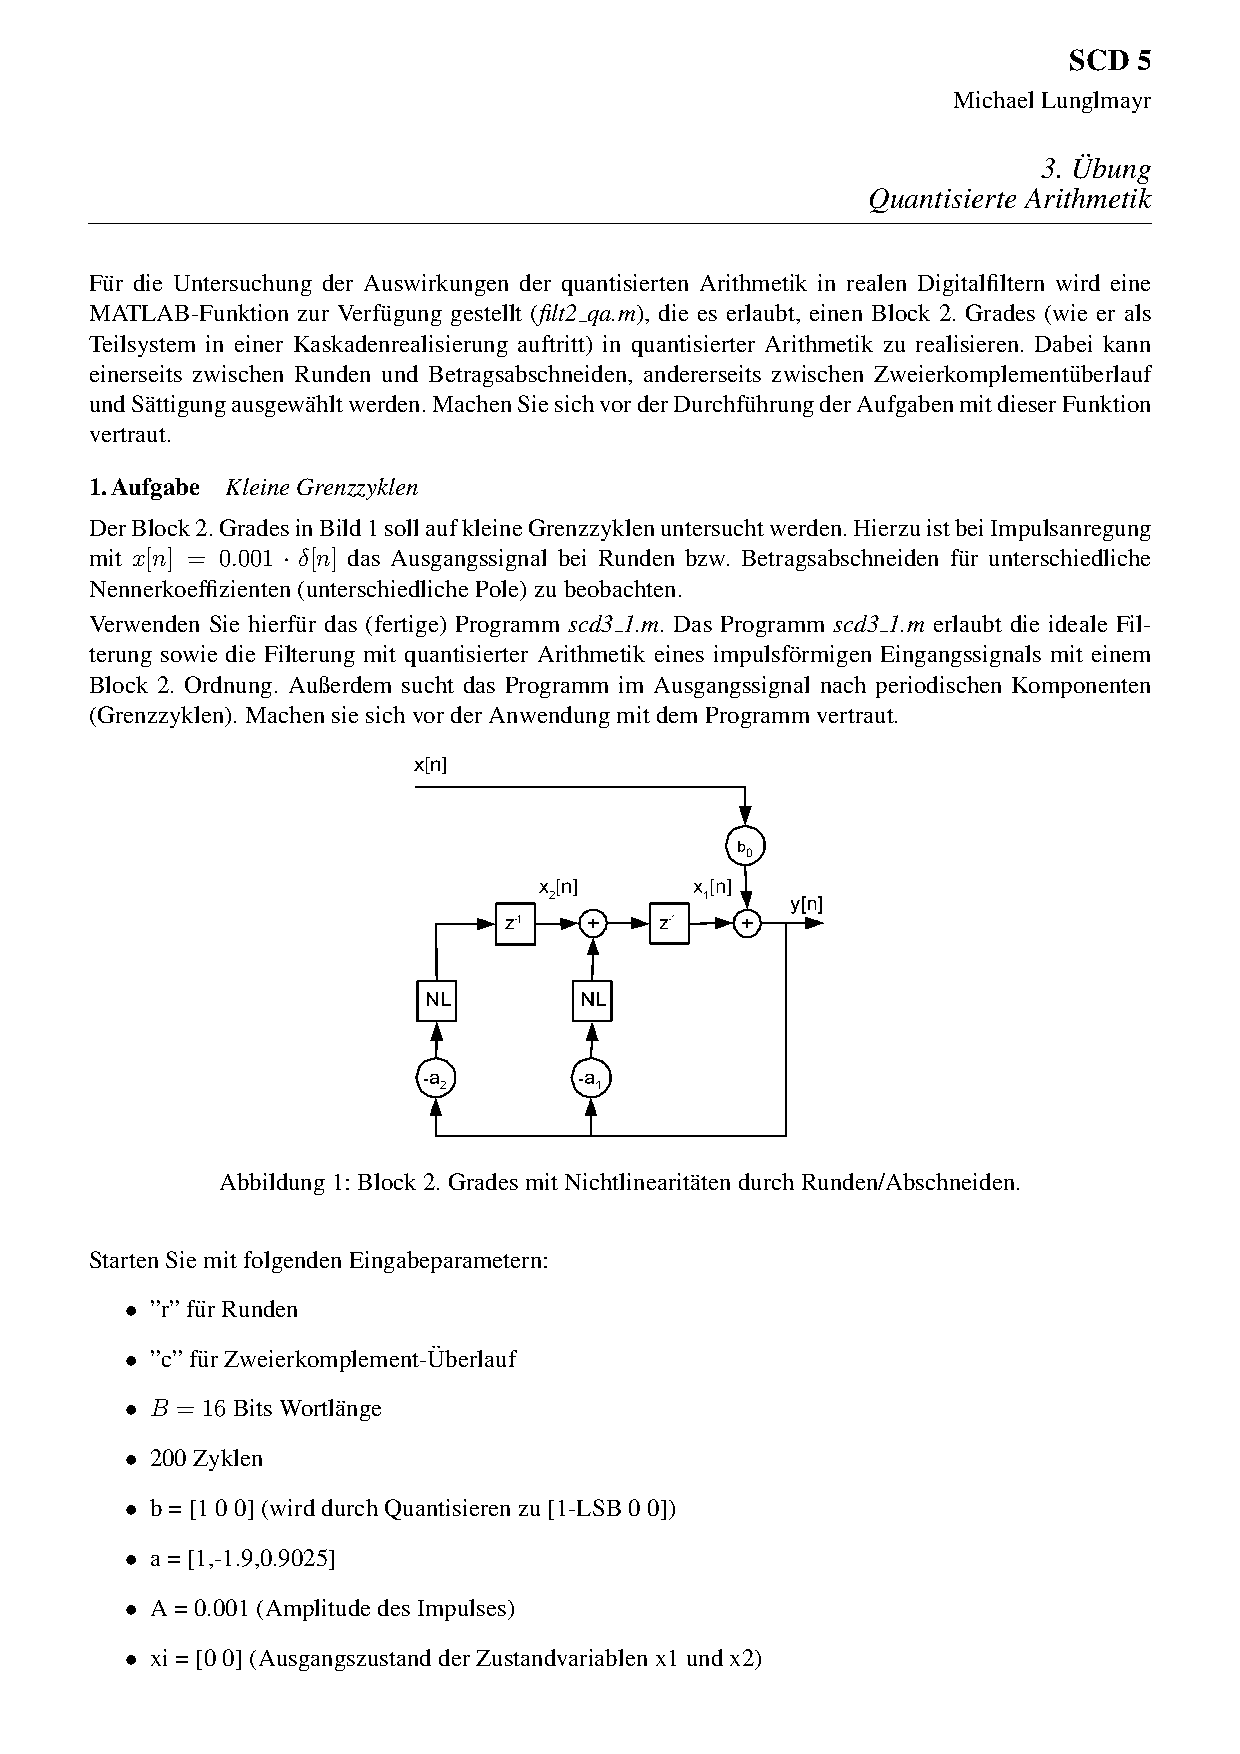
\includepdf[pages=-]{../SCD_UE03_Deckblatt.pdf}

\tableofcontents

\newpage

\section{Aufgabe 1 - Kleine Grenzzyklen}

\subsection{Grenzzyklen durch Runden}

\begin{center}
Abbildung 1.1.1: a = [1,-1.9,0.9025]\\
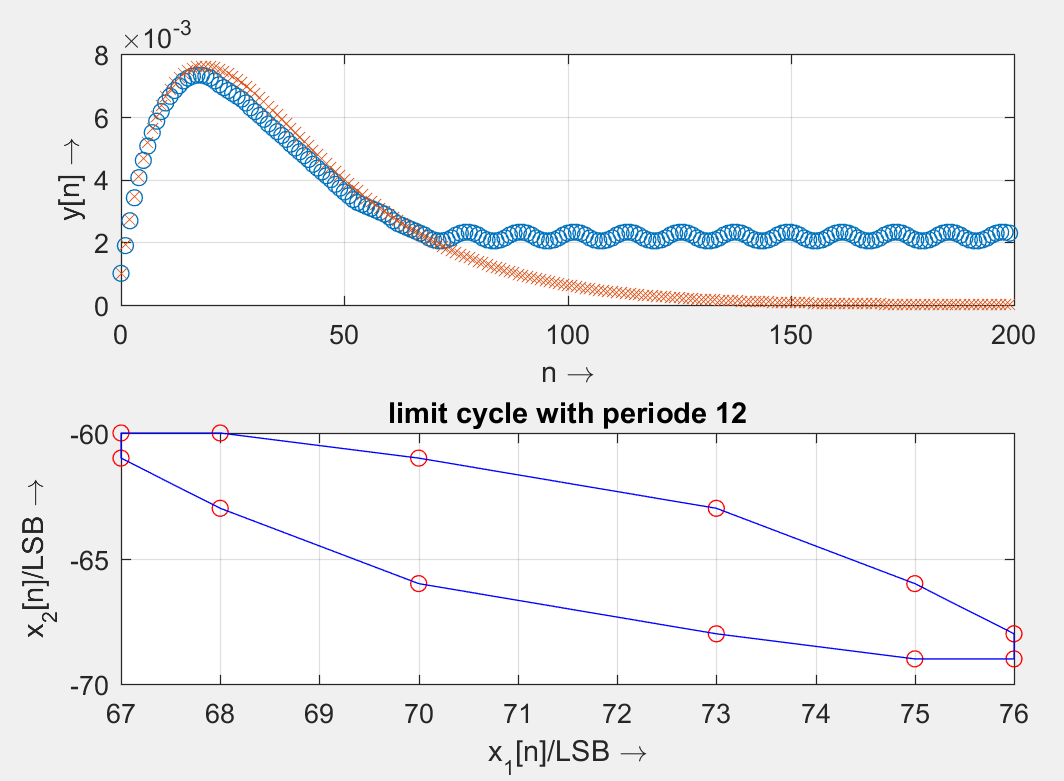
\includegraphics[scale=0.9]{../Tab1_1.PNG}
\end{center}

\begin{center}
Abbildung 1.1.2: a = [1,-1.6454,0.9025]\\
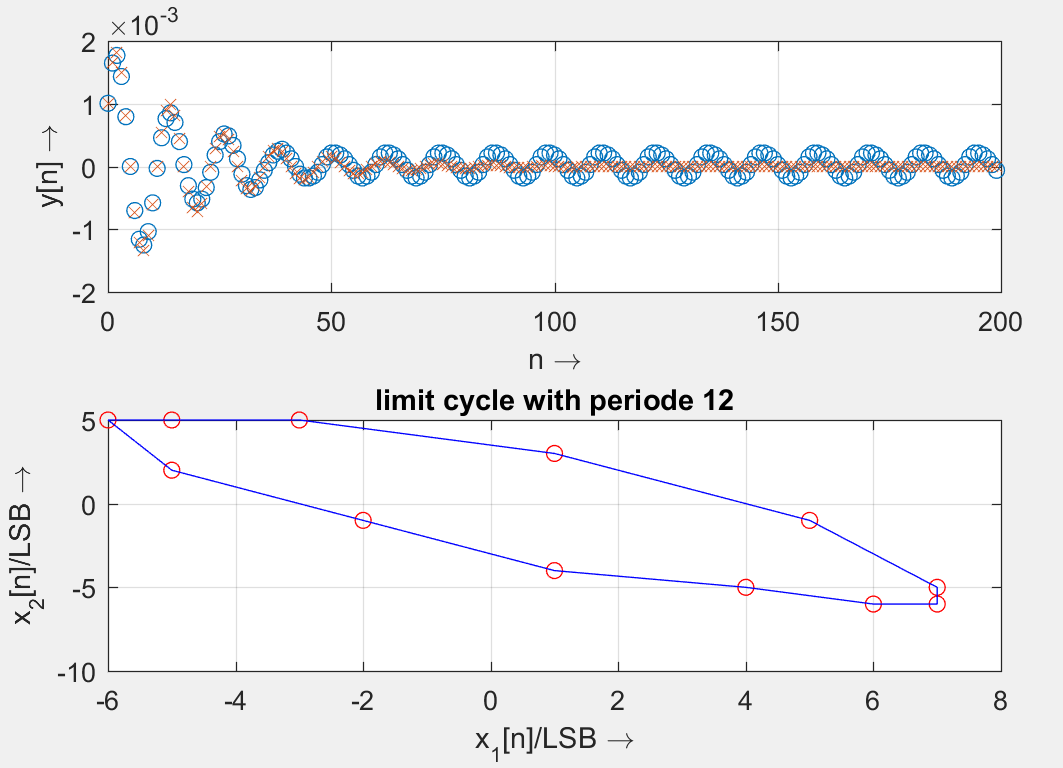
\includegraphics[scale=0.9]{../Tab1_2.PNG}
\end{center}

\newpage

\begin{center}
Abbildung 1.1.3: a = [1,-0.95,0.9025]\\
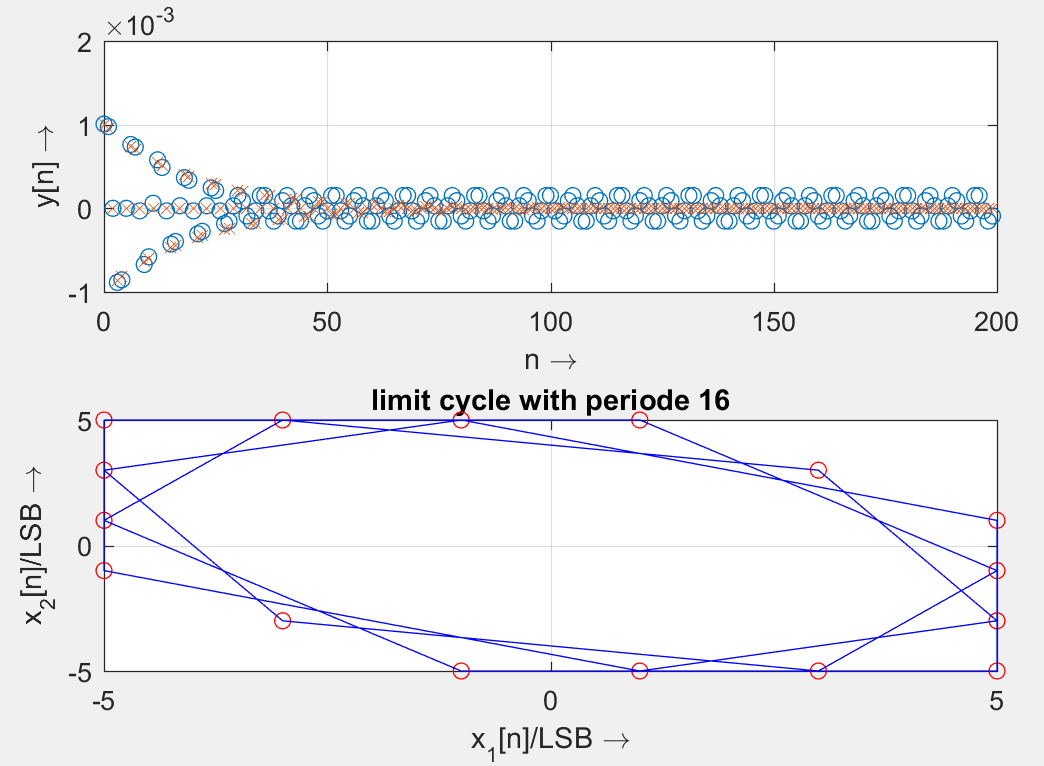
\includegraphics[scale=0.9]{../Tab1_3.PNG}
\end{center}

\begin{center}
Abbildung 1.1.4: a = [1,0,0.9025]\\
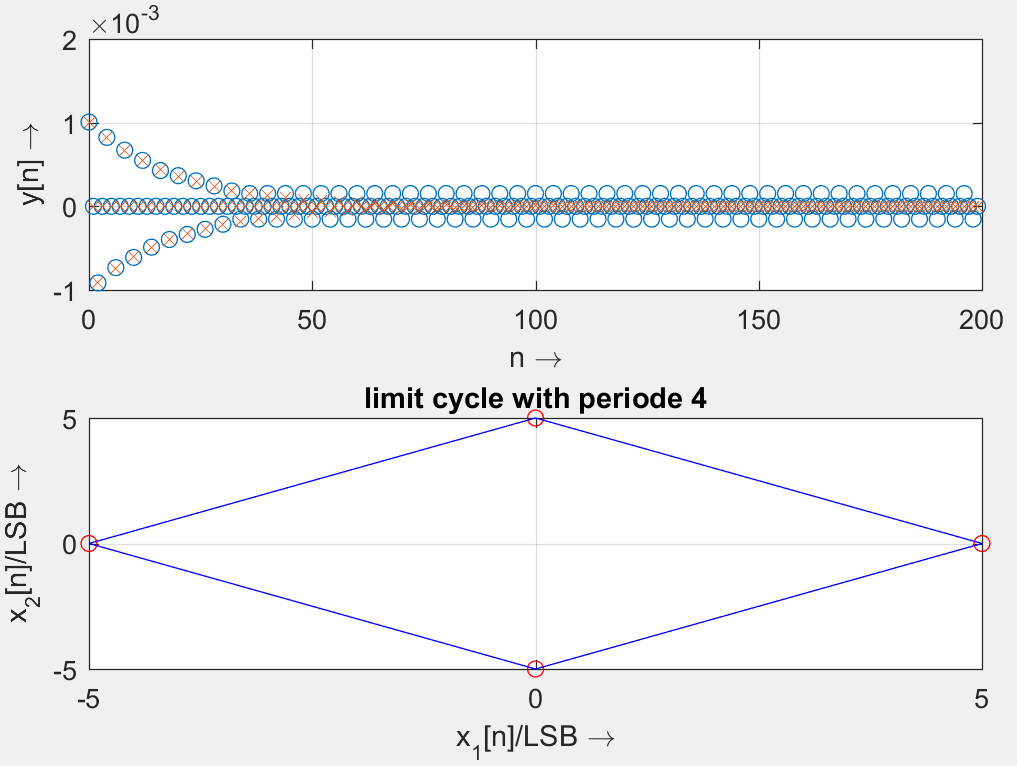
\includegraphics[scale=0.9]{../Tab1_4.PNG}
\end{center}

\newpage

\subsection{Grenzzyklen durch Betragsabschneiden}

\begin{center}
Abbildung 1.2.1: a = [1,-1.9,0.9025]\\
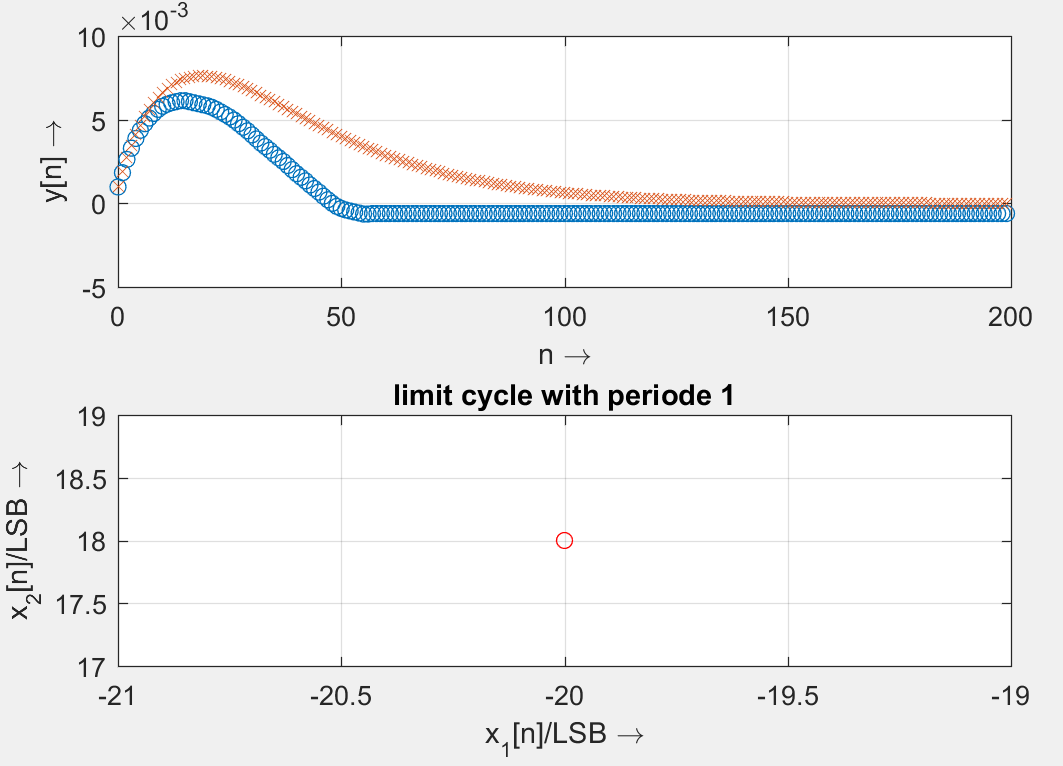
\includegraphics[scale=0.9]{../Tab2_1.PNG}
\end{center}

\begin{center}
Abbildung 1.2.2: a = [1,-1.6454,0.9025]\\
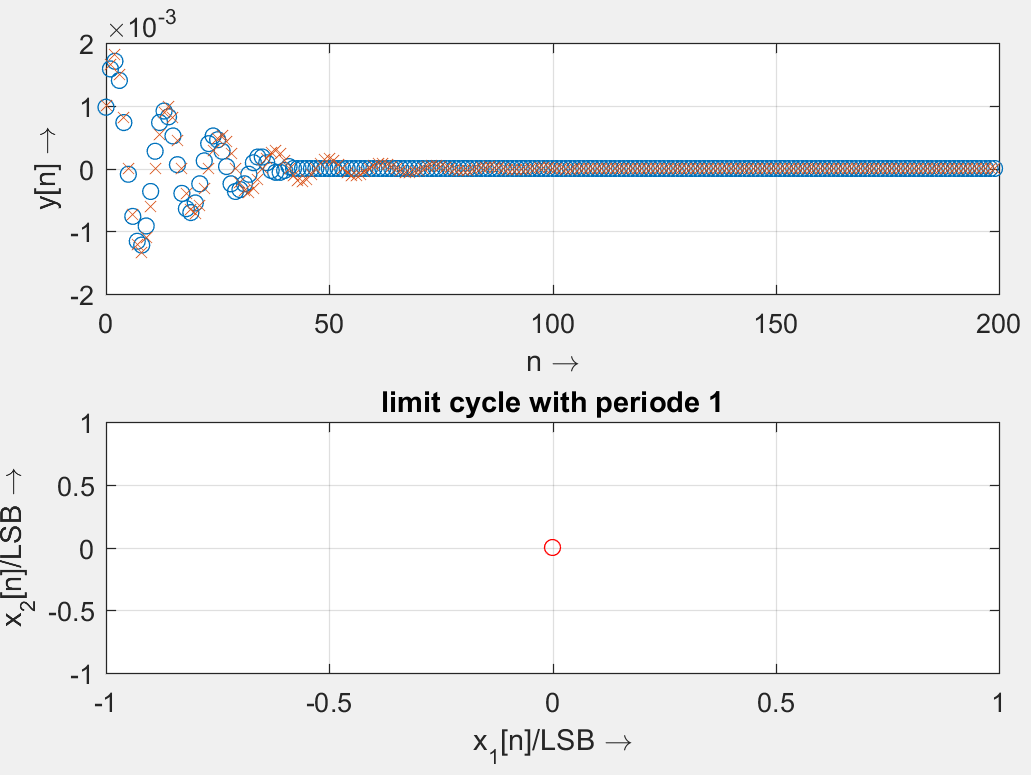
\includegraphics[scale=0.9]{../Tab2_2.PNG}
\end{center}

\newpage

\begin{center}
Abbildung 1.2.3: a = [1,-0.95,0.9025]\\
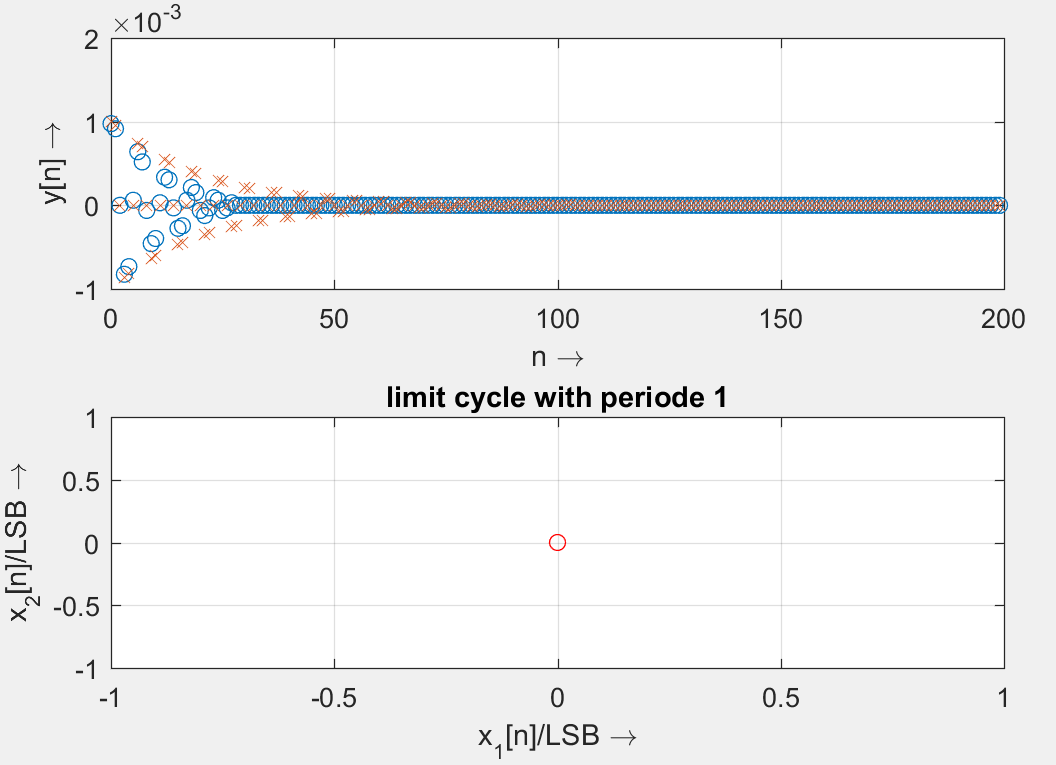
\includegraphics[scale=0.9]{../Tab2_3.PNG}
\end{center}

\begin{center}
Abbildung 1.2.4: a = [1,0,0.9025]\\
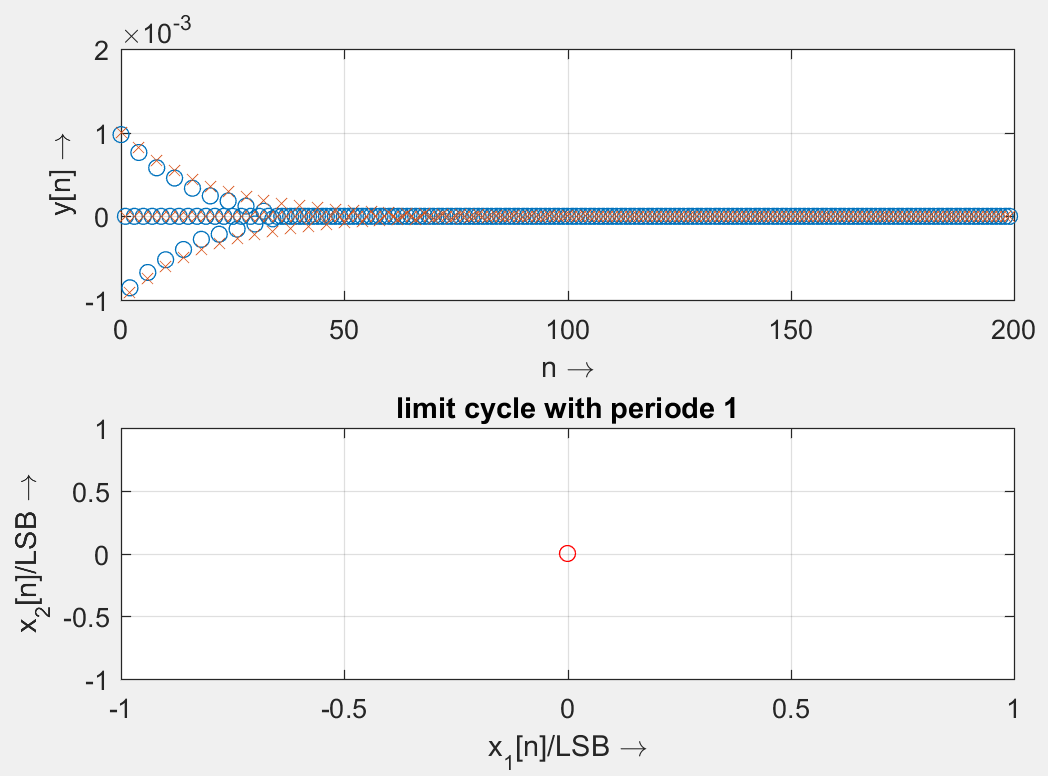
\includegraphics[scale=0.9]{../Tab2_4.PNG}
\end{center}

\subsection{Erkenntnis}

Es ist zu erkennen, das die kleinen Grenzzyklen nur durch Runden entstehen und bei Betragsabschneiden nicht auftreten.

\newpage

\section{Aufgabe 2 - Große Grenzzyklen}

\subsection{Grenzzyklen durch Betragsabschneiden}

\begin{center}
Abbildung 2.1: a = [1,-1.9,0.9025]\\
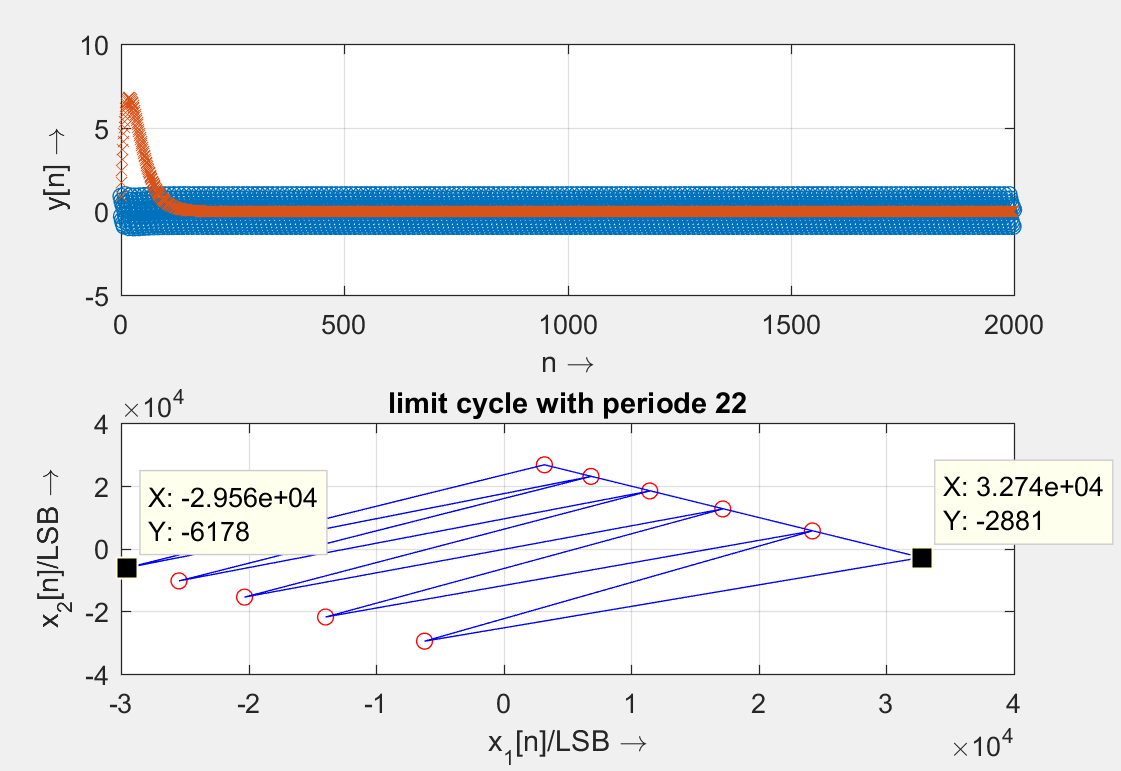
\includegraphics[scale=0.9]{../Tab3_1.PNG}
\end{center}

\begin{center}
Abbildung 2.2: a = [1,-1.6454,0.9025]\\
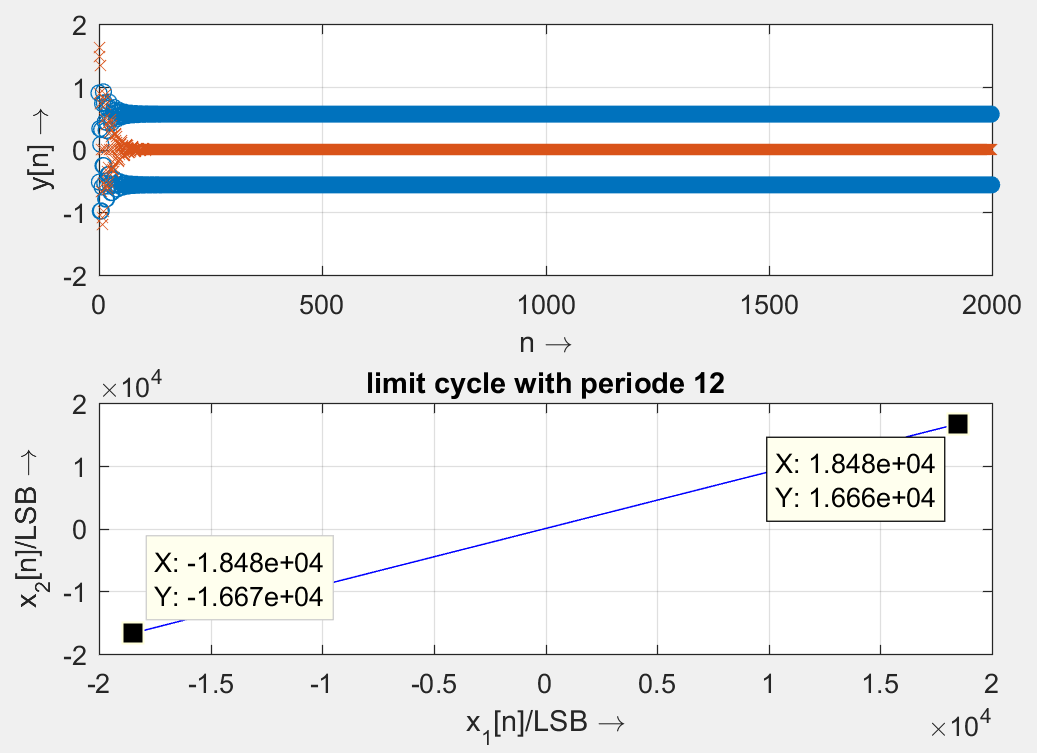
\includegraphics[scale=0.9]{../Tab3_2.PNG}
\end{center}

\newpage

\begin{center}
Abbildung 2.3: a = [1,-0.95,0.9025]\\
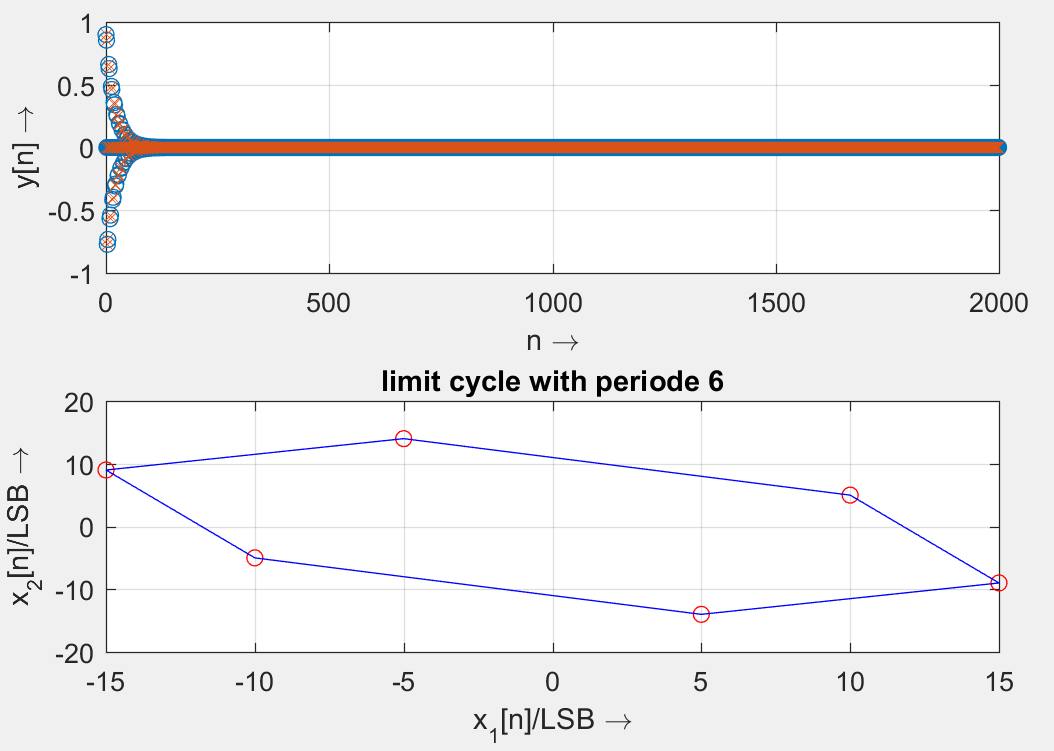
\includegraphics[scale=0.9]{../Tab3_3.PNG}
\end{center}

\begin{center}
Abbildung 2.4: a = [1,0,0.9025]\\
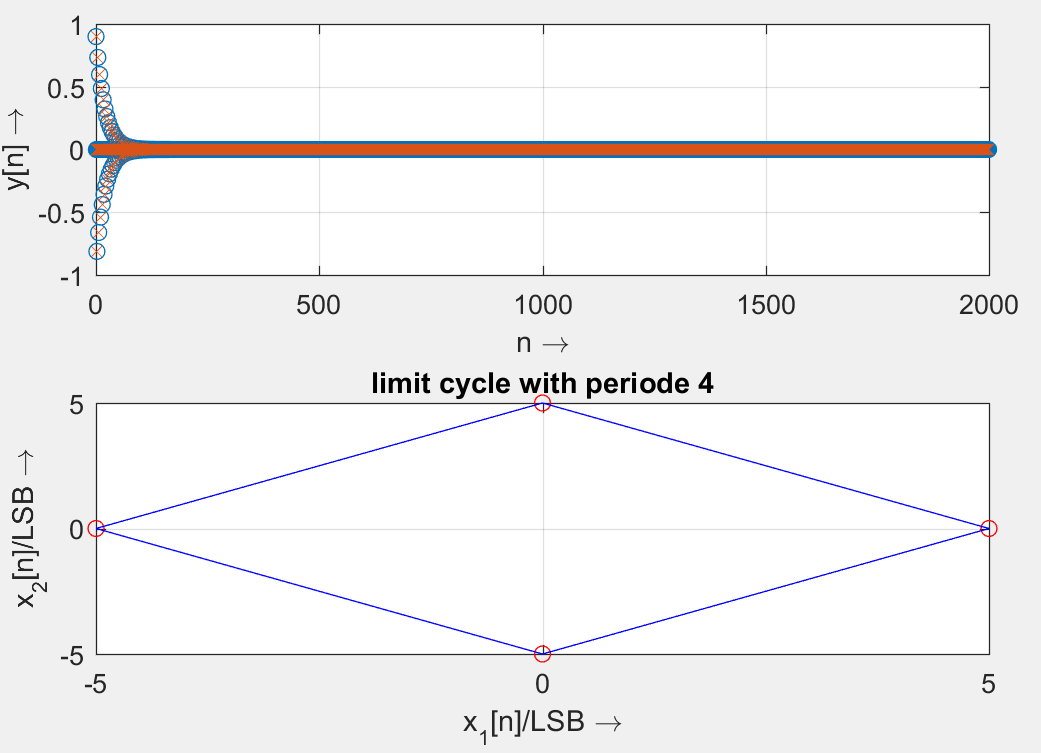
\includegraphics[scale=0.9]{../Tab3_4.PNG}
\end{center}

\subsection{Erkenntnis}

Es ist zu erkennen, das durch das Betragsabschneiden bei einem hohem Eingangsimpuls große Grenzzyklen entstehen. Je näher die Parameter dem Stabilitätsgrenzwert kommen, desto stärker ist die Schwingung die entsteht.

\newpage

\section{Aufgabe 3}

\subsection{Screenshots der Systeme bei B=14 und l1-Skalierung}

\begin{center}
Abbildung 3.1: a = [1,-1.9,0.9025]\\
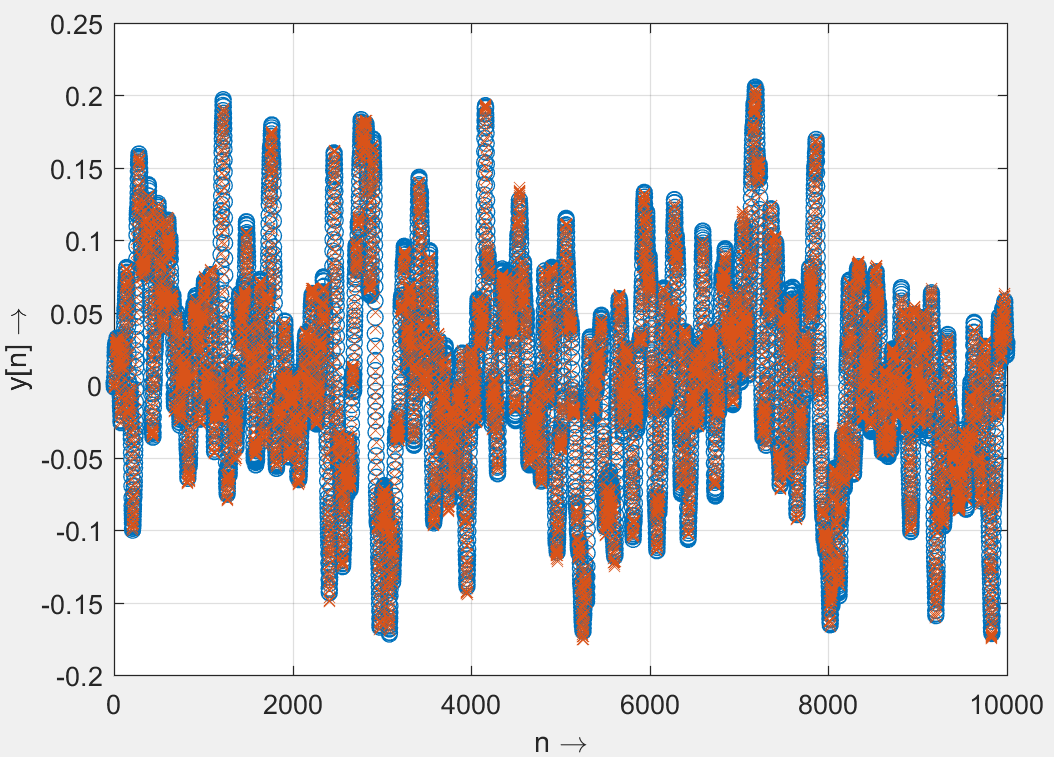
\includegraphics[scale=0.9]{../Tab4_1_14B_l1.PNG}
\end{center}

\begin{center}
Abbildung 3.2: a = [1,-1.6454,0.9025]\\
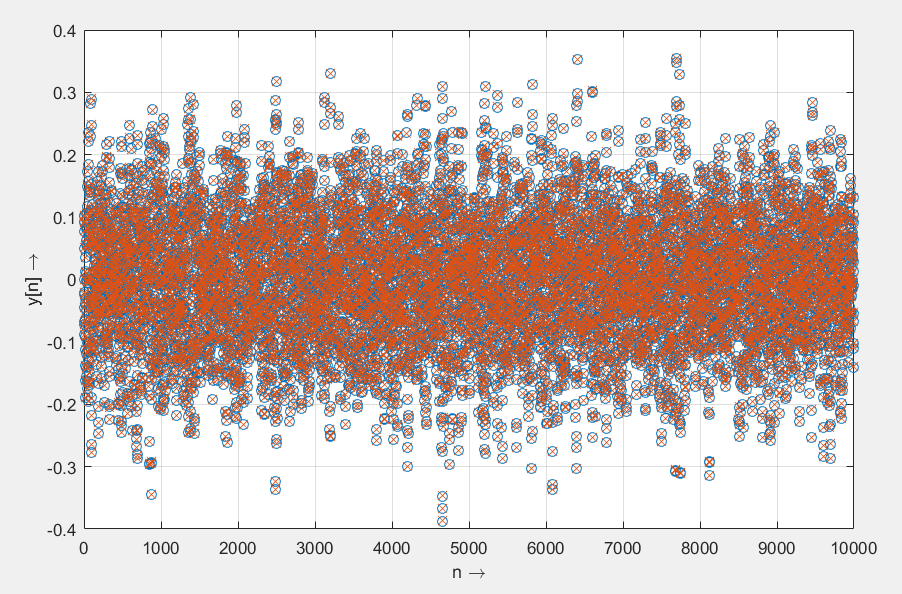
\includegraphics[scale=0.7]{../Tab4_2_14B_l1.PNG}
\end{center}

\newpage

\begin{center}
Abbildung 3.3: a = [1,-0.95,0.9025]\\
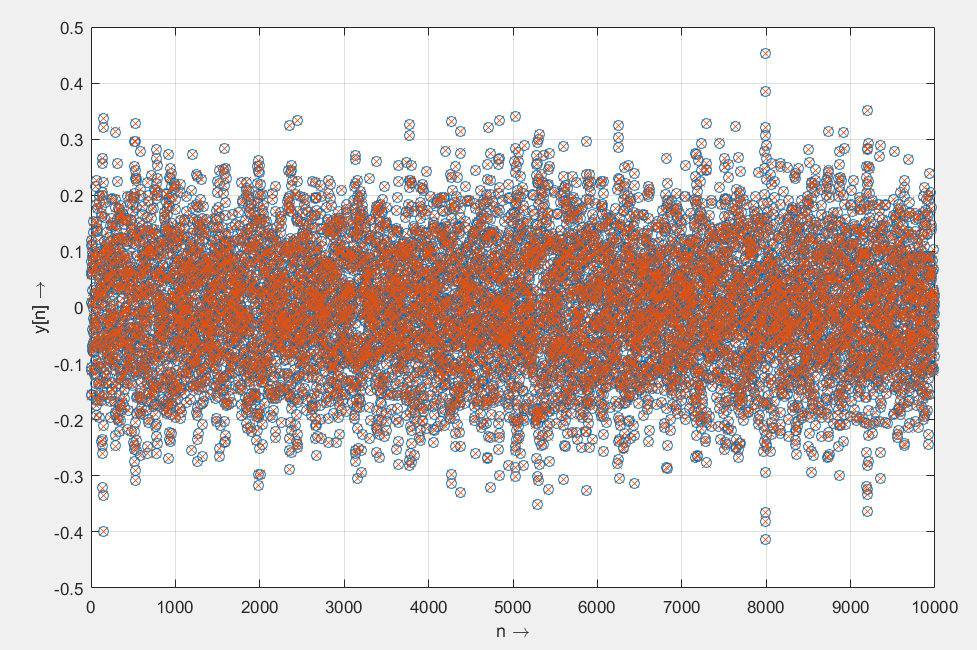
\includegraphics[scale=0.7]{../Tab4_3_14B_l1.PNG}
\end{center}

\begin{center}
Abbildung 3.4: a = [1,-0.0332,0.9025]\\
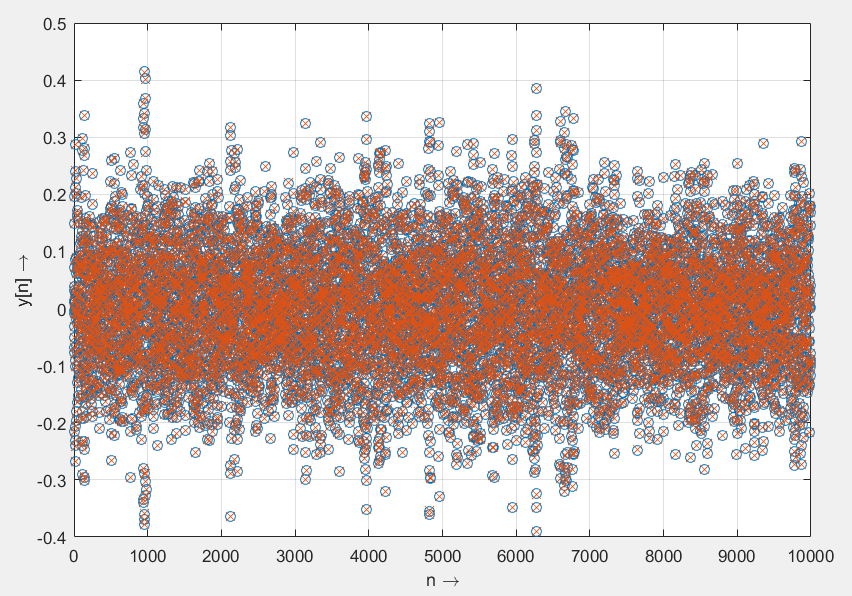
\includegraphics[scale=0.7]{../Tab4_4_14B_l1.PNG}
\end{center}

\newpage

\begin{center}
Abbildung 3.5: a = [1,0,0.9025]\\
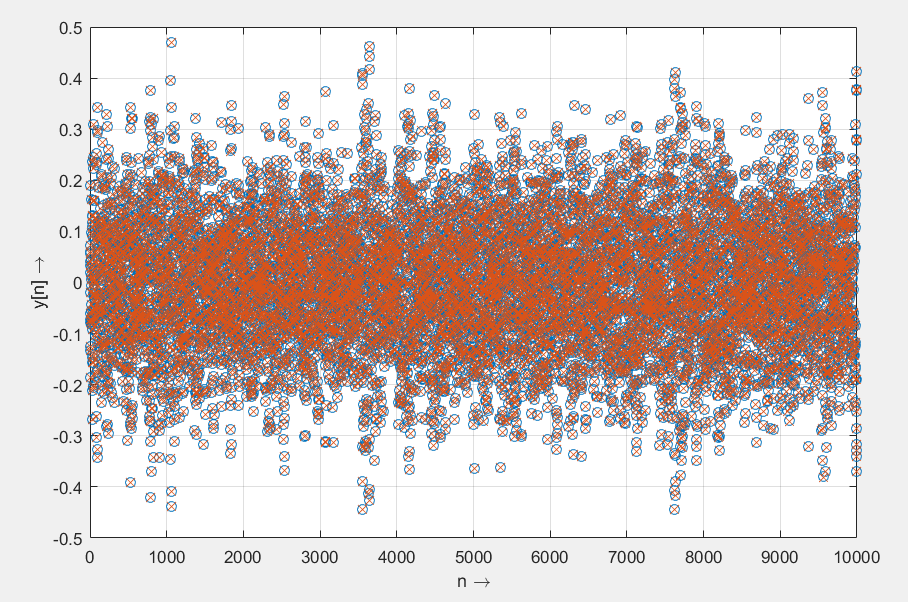
\includegraphics[scale=0.7]{../Tab4_5_14B_l1.PNG}
\end{center}

\subsection{Erkenntnis}

Besonders auffällig ist, dass die l2-Skalierung in diesen System beinahe keine Verbesserung bei erhöhter Bitanzahl bringt. Allgemein gesagt hat diese Skalierung in diesen Systemen keine besonderen Mehrwert. Weiters ähneln sich l1- und l\_inf-Skalierung sehr, zwischen diesen beiden gibt es auch fast keinen Unterschied. Es macht also keinen großen Unterschied, welche der beiden Skalierungen am Ende wirklich verwendet wird. In den letzten beiden Zeilen verbessert sich der SNR nochmals um einige dB, trotz der minimalen Änderung von a1 von -0.0332 auf 0.

\subsection{Bestimmung des maximalen SNR}

Zur Bestimmung des maximalen SNR wurde das bestehende Skript verändert und in eine for-Schleife verschachtelt, die den SNR für alle Skalierungsfaktoren von 0 bis 1 mit einer Auflösung von 0.001 berechnet und den größten Wert abspeichert. Als Eingangsdaten für die Schleife wurden immer die gleichen Zufallszahlen verwendet.

\begin{table}[H]
\centering
\begin{tabular}{|c|l|}
\hline
Nennerkoeffizienten                              & \multicolumn{1}{c|}{SNR bei Faktor s und 14 Bit} \\ \hline
\multirow{2}{*}{a = {[}1,-1.9,0.9025{]}}         & s = 0.011                                        \\
                                                 & 38.5525 dB                                       \\ \hline
\multirow{2}{*}{a = {[}1,-1.6454,0.9025{]}}      & s = 0.092                                        \\
                                                 & 56.2169 dB                                       \\ \hline
\multirow{2}{*}{a = {[}1,-0.95,0.9025{]}}        & s = 0.18                                         \\
                                                 & 62.0987 dB                                       \\ \hline
\multirow{2}{*}{a = {[}1.0000 -0.0332 0.9025{]}} & s = 0.202                                        \\
                                                 & 63.1923                                          \\ \hline
\multirow{2}{*}{a = {[}1,0,0.9025{]}}            & s = 0.224                                        \\
                                                 & 68.434 dB                                        \\ \hline
\end{tabular}
\end{table}

\end{document}